\section{Discussion}
\subsection{Performance Comparison}

All model performance are evaluated from both classification and retrieval viewpoints. Each baseline method is run on three graphs including the main graph, the sparse graph, and their combined graph. While my model can only be tested by utilizing both graphs. Table \ref{tab:c4_evaluation} shows the overall model performance under three graphs. Particularly, I run my model ten times and report the average performance result. To verify my model's superiority, I calculate the performance differences between my model and the best baseline on each metric for all the runs, and apply a pairwise t-test to check whether the performance difference is significant.

Our model output is a predicted score in the range from 0 to 1. Its associated label is assigned to be one of ``\textit{closer}'', ``\textit{similar}'' or ``\textit{farther}'' based on which third the predicted score lies in (associated with label definition in Section \ref{sc:pcd}). For example, a user triplet $\langle u_i,u_j,u_k \rangle$ with score 0.3 will be labelled as ``\textit{farther}'', which means compared with $u_k$, $u_j$ is has a farther community closeness to $u_i$. After that, from classification perspective, ACC, F1 and MCC scores are calculated by comparing predicted labels with the ground truth labels. While from retrieval perspective, MRR, NDCG and MAP are calculated for the pairwise ranking within user triplets.

Table \ref{tab:c4_evaluation} shows that all baseline performances in the combined graph achieve the best among three types of graphs. And performances in the main graph are always better than in the sparse graph. It demonstrates that main graph holds beneficial information to reveal user potential communities in sparse graphs. The random baseline is with similar performance among all three graphs, which makes sense because the random community partition is regardless of graph structures. It can be used as the default model to compare with in each graph. For the rest six baselines, random walk based baselines (Infomap and LSH) do not perform well in all three graphs. Their evaluation results are just a bit better than random model performance. WMW model performs the best among all baselines. Actually, its results are always the best in three graphs of both datasets. However, by taking the pairwise t-test, it statistically proves that my model still significantly outperforms the WMW model in terms of all metrics. 

It is also interesting to see that the model evaluation results are consistent in all datasets. For example, DNR model always performs better than LSH model. The only exception is that BigClam performs better than Node2vec in SH-NE dataset, but worse in SH-CO dataset. 


\subsection{Ablation Study}
\begin{table}[h]
	%	\scriptsize
	
	% 	\small
	\centering
%	\renewcommand{\tabcolsep}{3pt}
	%	\renewcommand\arraystretch{0.5}
	\begin{tabular}{|c|c|c|c|c|c|c|c|} 
		\hline
		\textbf{Dataset}& \textbf{Model}	
		& \textbf{ACC}& \textbf{F1}& \textbf{MCC}& \textbf{MRR} & \textbf{NDCG}& \textbf{MAP}\\ \hline
		\multirow{5}{*}{ \textbf{SH-NE}} & -- RCR  &-2.61&-2.51&-3.76&-0.73&-0.54&-0.96\\
		& -- DTR &-1.32&-1.49&-2.96&-1.01&-0.14&-0.57\\ 
		& -- NF &-17.31&-17.01	&-25.92&-5.35&-3.88&-6.05\\
		& -- CF &-7.94&-8.48&-11.71&-2.61&-1.92&-3.01\\
		& -- CC &-2.15&-2.05&-3.08&-0.49&-0.35&-0.65\\ 
		& -- MT &-2.43&-2.55&-4.82&-0.78&-0.82&-1.24\\ 
		\hline
		\multirow{5}{*}{ \textbf{SH-CO}} & -- RCR &-2.13&-2.45&-3.07&-1.65&-0.58&-0.79  \\  
		& -- DTR &-3.45&-2.89&-1.95&-2.22&-0.43&-0.88\\ 
		& -- NF &-26.13&-25.83&-39.97&-9.81&-7.50&-19.35\\ 
		& -- CF &-21.12&-5.53&-8.45&-2.03&-1.50&-2.50\\
		& -- CC &-4.32&-4.34&-6.57&-1.56&-1.24&-1.91\\
		& -- MT &-1.32&-1.24&-2.66&-0.33&-0.21&-0.45\\ \hline
	\end{tabular}
	% 	\vspace{-0.5em} 
	\caption{Performance differences on all evaluation metrics between each ablated model and the original model. ``-'' refers to remove related component from my model. Results are scaled in percentage (\%).}
	\label{tab:c4_ablation}
	% 	\vspace{-1em} 
\end{table} 
In this section, I aim to explore whether all components of my proposed model have positive effect on final model performance and which component has the largest impact. There are six components that can be disassembled from the main model, including Raw Community Representation in the main graph (RCR), Direct Transformation Representation (DTR), Node-level filter (NF), Community-level filter (CF), Community Constraint (CC) and Masked Training (MT). I iteratively remove each component while keep the rest firmed to demonstrate their performance difference compared to the original model. All comparison results are showed in Table \ref{tab:c4_ablation}.


Among the six components, if I remove node-level filter, the performance drop dramatically, even worse than some of baseline models. It indicates that node-level information are excessive and noisy. Without appropriate filtering on the propagated information, it would vitally pollute the quality of user representations. Similarly,  community-level filter also has a huge impact on model performance, meaning filtering propagated information from a coarser view also has a positive effect on learning user representations. By contrast, the two extra representations (RCR and DTR) do not have strong influence in my model. Having these information can slightly improve model performance as they still involve extra information. However, as one-hot embeddings, the amount of new information that RCR can offer is very limited. Similarly, DTR is only one-layer transformation on multi-hot embeddings. The information it can offer is also limited. By adding extra constraint, CC also has a little positive effect to enhance model performance. But as I always set its weight with a small value in training process, its influence is also indifferent. MT has the least impact on model performance as randomly masking user behaviors in the main graph has an overlapped effect with attentive weights calculated from the node-level filter in Section \ref{sc:upr}.

\subsection{User-Type Analysis}
\label{sc:ua}
\begin{table}[h]
	%	\scriptsize
	
	% 	\small
	\centering
%	\renewcommand{\tabcolsep}{3.5pt}
	%	\renewcommand\arraystretch{0.5}
	\begin{tabular}{|c|c|c|c|c|c|c|c|} 
		\hline
		\textbf{Dataset}& \textbf{User}	
		& \textbf{ACC}& \textbf{F1}& \textbf{MCC}& \textbf{MRR} & \textbf{NDCG}& \textbf{MAP}\\ \hline
		\multirow{3}{*}{ \textbf{SH-NE}} & MU & 0.7132 & 0.7133 & 0.6012&  0.9112 & 0.9324 & 0.8704  \\   
		& MO & 0.6356 & 0.6477 & 0.4780&  0.8739 & 0.9002 & 0.8418 \\
		& SO & 0.6009 & 0.6117 & 0.4324&  0.8600 & 0.8988 & 0.8393 \\
		\hline
		\multirow{3}{*}{ \textbf{SH-CO}} & MU & 0.7852& 0.7780& 0.6724& 0.9300& 0.9474& 0.9015 \\   
		& MO & 0.7334& 0.7565& 0.6601& 0.9012& 0.9400& 0.8874\\
		& SO & 0.6823& 0.6915& 0.6844& 0.8990& 0.9222& 0.8789 \\\hline
	\end{tabular}
	% 	\vspace{-0.5em} 
	\caption{Three types of user performance in two datasets.}
	\label{tab:ua}
	% 	\vspace{-1em} 
\end{table} 

As aforementioned in Section \ref{sc:dataset}, there are three types of users in my cross-graph datasets including \textit{MU} (mutual users appeared in both graphs),  \textit{MO} (users only appeared in the main graph), and  \textit{SO} (users only appeared in the sparse graph). Unlike my training data which is constructed only with mutual users, my testing data can be with all types of users. To examine my model performance on each type of users, user triplets with only single type of users are screened, i.e., an eligible user triplet only contains three \textit{MO} type users. In fact, the performance on \textit{MO} user triplets reflects the capability of my model to solve cold-start problem as these users have no behaviors in the sparse graphs. The result showed in Table \ref{tab:ua} demonstrates that the label of \textit{MU} triplets can be best identified, which makes sense as the information of mutual users come from both graphs. While performance results on \textit{MO} are better than \textit{SO} user triplets, which might because that users are likely to have more enriched behaviors in the main graph compared with the sparse graph. Even that, the performance of my model on \textit{SO} user triplets is still better than most of baselines running on the combined graph.

\subsection{Graph Sparsity Influence}
\begin{figure}
	%\hspace*{-1cm} 
	\centering
	%%\subfloat[BLEU]{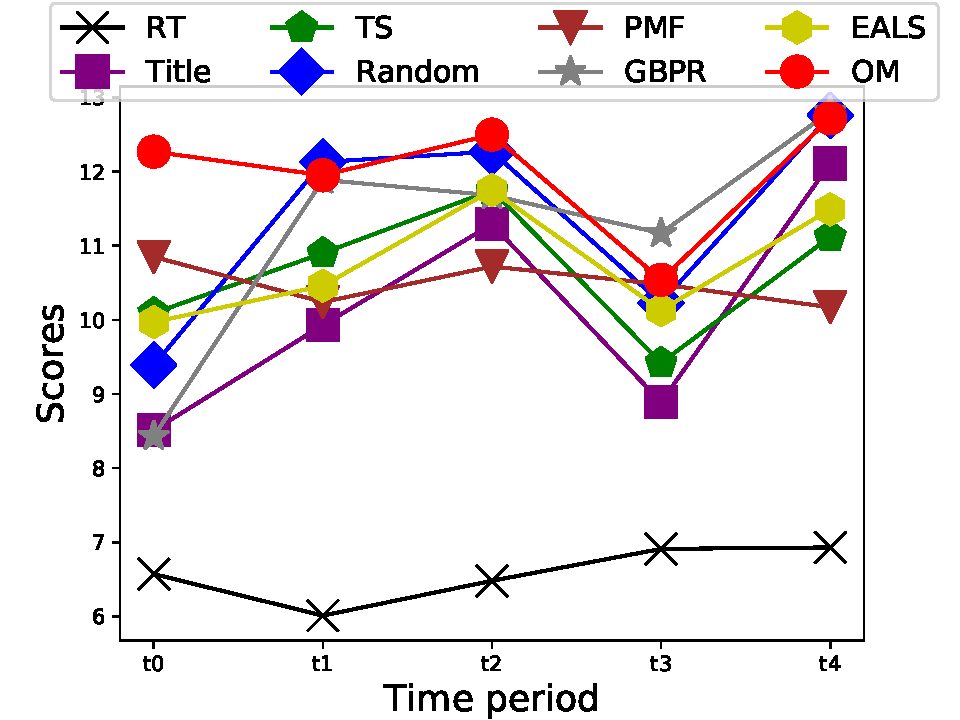
\includegraphics[width = 1.5in]{img/bleu.pdf}}  
	\subfloat[ACC]{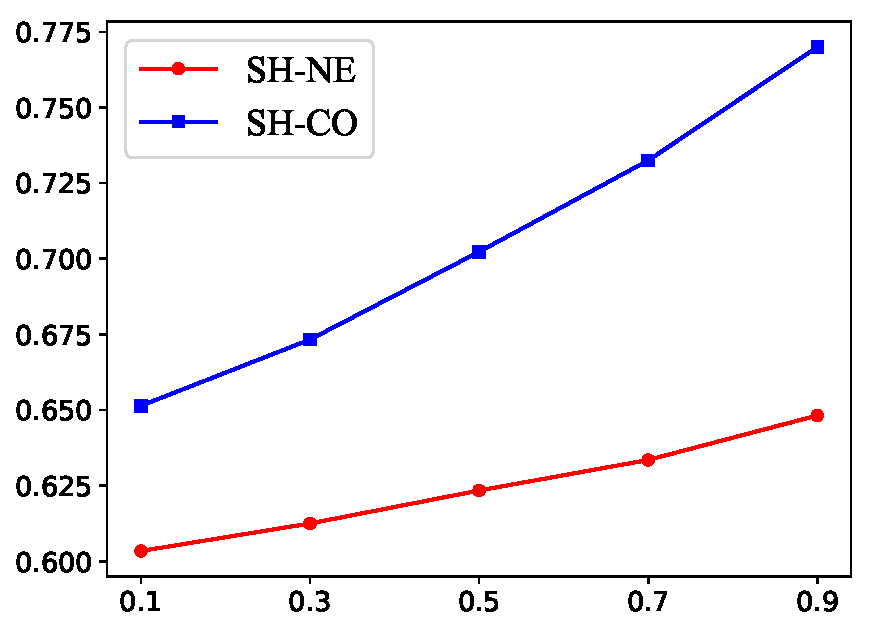
\includegraphics[width = 2in]{img/chapter4/acc.pdf}} 
	\subfloat[F1]{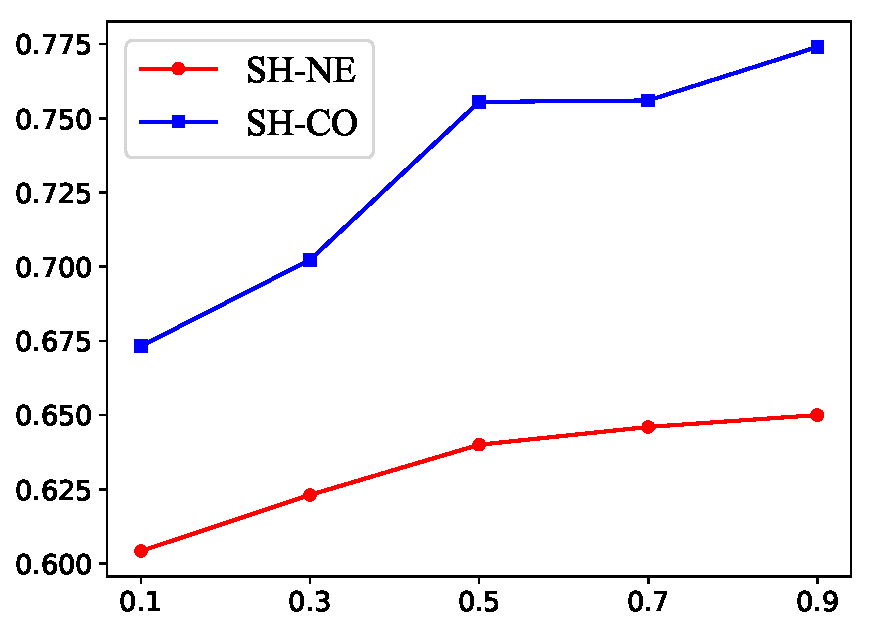
\includegraphics[width = 2in]{img/chapter4/f1.pdf}} 
	\subfloat[MCC]{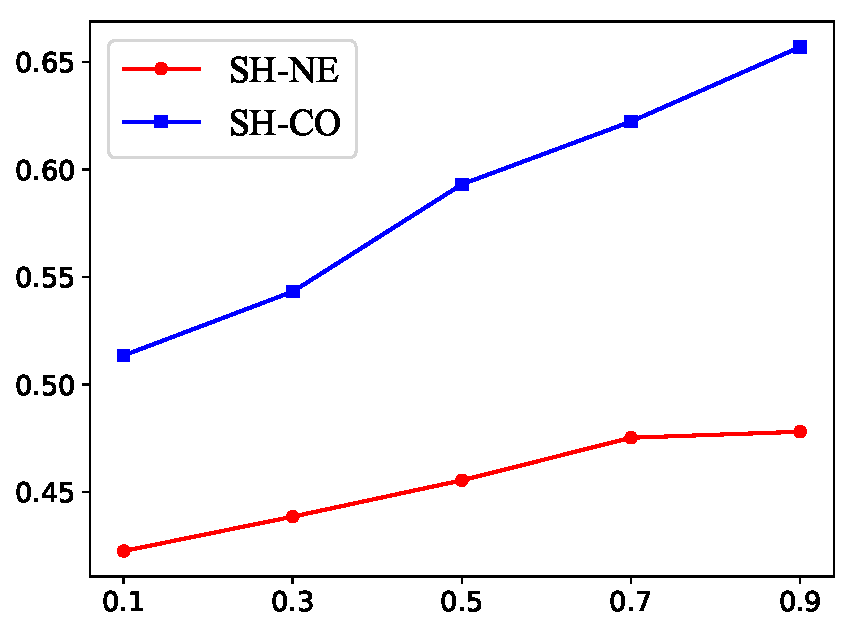
\includegraphics[width = 2in]{img/chapter4/mcc.pdf}}\\ 
	\subfloat[MRR]{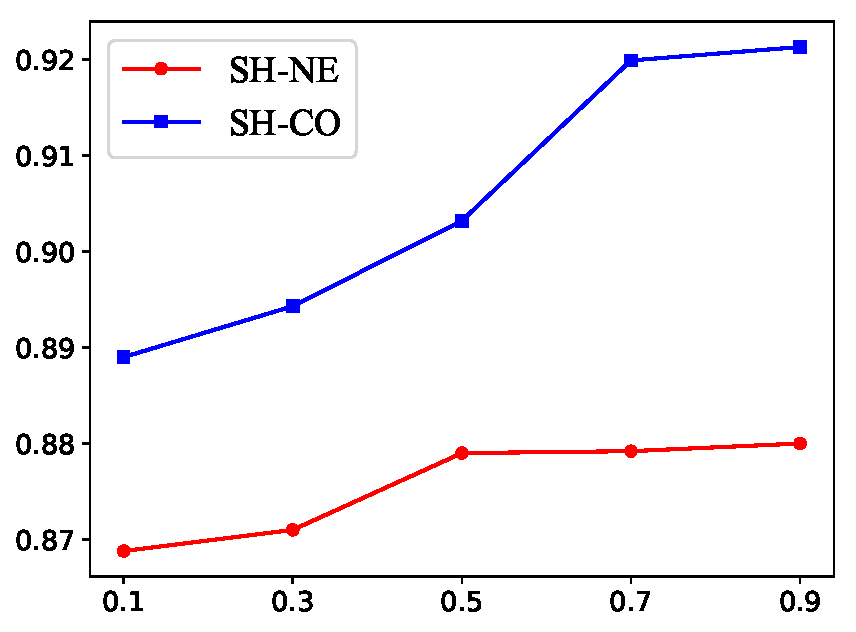
\includegraphics[width = 2in]{img/chapter4/mrr.pdf}} 
	\subfloat[NDCG]{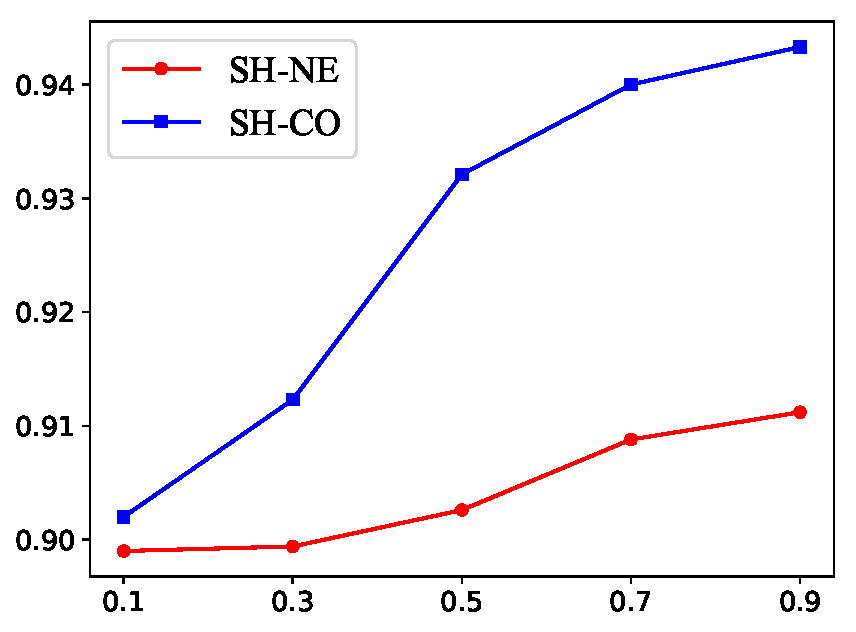
\includegraphics[width = 2in]{img/chapter4/ndcg.pdf}} 
	\subfloat[MAP]{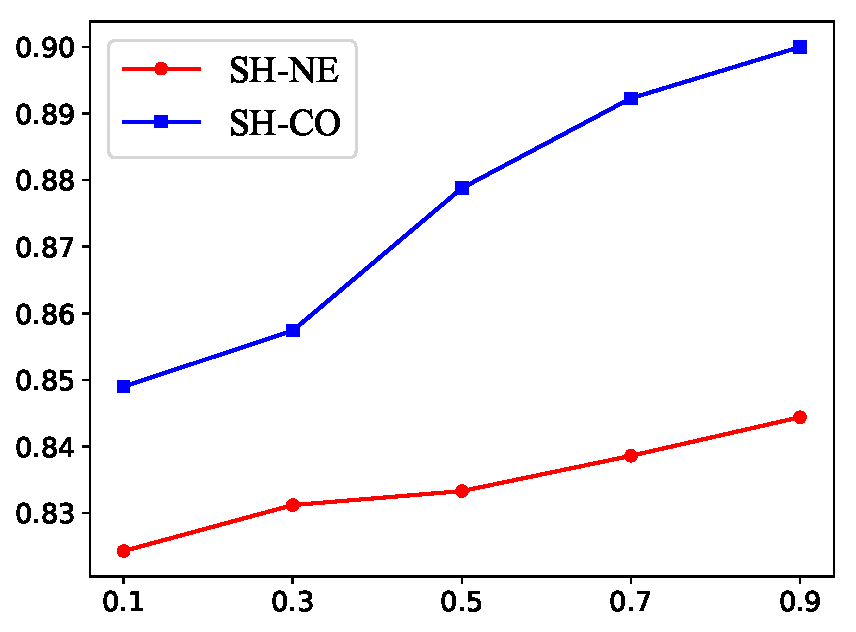
\includegraphics[width = 2in]{img/chapter4/map.pdf}} 
	\caption{Our model performance on all metrics under different graph sparsity scales. X-axis is the ratio of links preserved in the sparse graph. Y-axis is related metric score.}
	% 	 \vspace{-1em}
	\label{fig:sparsenss}
	% 	\vspace{-1em} 
\end{figure}
To explore my model robustness on graph sparsity, I randomly keep $\delta$ ratio of the total links in the sparse graph, where  $\delta=\{0.1,0.3,0.5,0.7,0.9\}$. My model is trained on the whole main graph and each truncated sparse graph. The reported evaluation metrics under all sparse graphs with varied scales are visualized in Figure \ref{fig:sparsenss}. All metrics in both SH-NE and SH-CO datasets are in a rising trend with more links preserved in related sparse graphs. Compared with SH-NE dataset, SH-CO can benefit more from the sparse graph as it has a larger increase in all reported metrics. 

With more links are preserved, all evaluation metrics first grows rapidly. While the increasing speed slows down when 70\%-90\% links are preserved. This phenomenon can be seen in almost all plots in Figure \ref{fig:sparsenss}. It can be explained by the law of diminishing marginal utility, meaning that the marginal utility to bring new information derived from each additional link is declined.

Although classification related  metrics significantly increase with more links preserved (i.e., F1 score in SH-CO dataset increases 10\% when involving sparse graph), the retrieval related metrics (MRR, NDCG and MAP) do not change much in the mean time. One possible reason is that the information from the main shopping graph already contains enough information for the pairwise ranking in user triplets. For example, without considering sparse graph information, my model has already achieved high MRR score as 0.87 in SH-NE dataset and 0.89 in SH-CO dataset, which is already better than most baseline results running on the combined graph.


\subsection{Case Study}

In order to testify whether my proposed Community Recurrent Unit is able to accurately calculate user affiliation scores in each community, I choose three users (labelled from user $u_1$ to user $u_3$) and calculate their affiliation scores of ten selected communities (labelled from community $c_1$ to community $c_{10}$) in the main shopping graph. The detailed result is visualized in Figure \ref{fig:case}. In the left part of the figure, darker color indicates higher affiliation scores in the range from 0 to 1. Besides, in the shopping graph, I also extract all products purchased by each user, and manually select the most representative ones summarized as keywords in a table, which is demonstrated in the right part of Figure \ref{fig:case}.

From the right-part table, $u_1$ and $u_2$ share similar shopping interests in clothing products. $u_2$ is more like a girl fond of sports. And $u_1$ more tends to be a fashion girl. While the shopping interests of $u_3$ is much far away from the other users. All purchased products by $u_3$ is furnishing stuffs. It seems s/he is decorating her/his living space. Referring to the left part of Figure \ref{fig:case}, the affiliation distribution among ten communities between $u_1$ and $u_2$ are very similar. They both have a high weight in community $c_1$, $c_7$ and $c_8$. While the community distribution of $u_3$ is totally different. $u_3$ is heavily affiliated with community $c_2$. The results of my calculated community affiliation distribution is consistent with actual user behaviors, which indicates my Community Recurrent Unit (CRU) is  functional well to reflect user community information.
\begin{figure}  
	% \advance\leftskip-1cm 
	\centering
	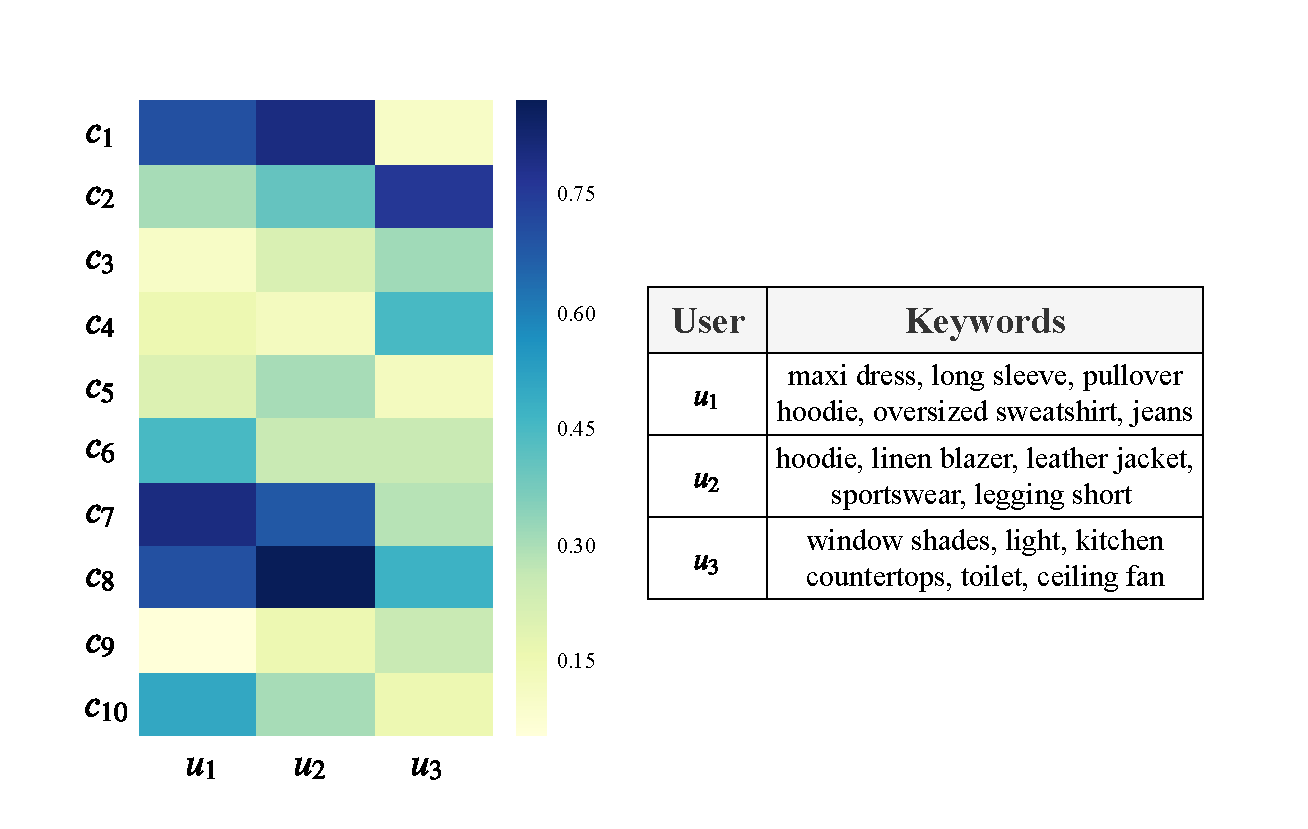
\includegraphics[width=1\columnwidth]{img/chapter4/case.pdf}
	%  \vspace{-3em}
	\caption{The left part shows ten community affiliation scores of three selected users in the shopping graph. The right part shows the keywords of their purchased products.}
	
	\label{fig:case}
	%  \vspace{-1em} 
\end{figure}

\begin{sidewaystable}[h]
	%	\scriptsize
	
	% 	\small
	\centering
	\renewcommand{\tabcolsep}{2.5pt}
	%	\renewcommand\arraystretch{0.5}
	\begin{tabular}{|c|c|c|c|c|c|c|c|c|c|c|c|c|c|} 
		\hline
		\multirow{2}{*}{ \textbf{Graph}} & 	\multirow{2}{*}{\textbf{Model}}	&\multicolumn{6}{c|}{\textbf{SH-NE Dataset}} & \multicolumn{6}{c|}{\textbf{SH-CO Dataset}}\\
		\cline{3-14}
		& & \textbf{ACC}& \textbf{F1}& \textbf{MCC}& \textbf{MRR}& \textbf{NDCG}& \textbf{MAP} & \textbf{ACC}& \textbf{F1}& \textbf{MCC} & \textbf{MRR}& \textbf{NDCG}& \textbf{MAP} \\ \hline
		\multirow{7}{*}{\textbf{Main }} &random  & 0.3324& 0.1677&-0.0001&0.7719&0.8373&0.7299&0.3302&0.1700&0.0027&0.7842&0.8444&0.7401\\ 
		& Infomap &0.3700& 0.2731&0.1201&0.8334&0.8421&0.7299 &0.3811&0.3723&0.1000&0.7888&0.8419&0.7430\\  
		& DNR &0.4210&0.4022&0.1789&0.8000&0.8366&0.7473&0.5194&0.5122&0.2712&0.8099&0.8773&0.7592\\   
		& LSH &0.3798&0.3813&0.0888&0.8002&0.8433&0.7328&0.4000&0.4123&0.1277&0.7812&0.8329&0.7570\\ 
		& Node2vec& 0.4888 &0.5014&0.2521&0.8229&0.8744&0.7832&0.5959&0.5832&0.3895&0.8422&0.8936&0.8222\\   
		& BigClam &0.5555&0.5399&0.3349&0.8421&0.8890&0.8024&0.5301&0.5334&0.3290&0.8335&0.8573&0.8005\\ 
		& WMW &0.6032&0.6158&0.4111&0.8632&0.8988&0.8256&0.6489&0.6661&0.5001&0.8789&0.9032&0.8499\\ \hline
		\multirow{7}{*}{\textbf{Sparse}} &random  & 0.3333& 0.1785&0.0003&0.7815&0.8438&0.7419&0.3301&0.1720&0.0030&0.7801&0.8400&0.7338\\ 
		& Infomap &0.3455& 0.1929&0.0031&0.7843&0.8399&0.7437 &0.3676&0.3211&0.0422&0.7905&0.8446&0.7401\\  
		& DNR &0.4433&0.4407&0.2020&0.8313&0.8678&0.7742&0.5273&0.5289&0.2787&0.8293&0.8765&0.7980\\   
		& LSH &0.3889&0.3917&0.0942&0.8008&0.8528&0.7343&0.4093&0.4177&0.1138&0.7833&0.8438&0.7404\\ 
		& Node2vec& 0.4849 &0.4958&0.2467&0.8219&0.8664&0.7774&0.5732&0.5746&0.3898&0.8412&0.8823&0.8146\\   
		& BigClam &0.5277&0.5355&0.3332&0.8441&0.8750&0.8005&0.5282&0.5280&0.3339&0.8298&0.8399&0.8033\\ 
		& WMW &0.5814&0.5900&0.3988&0.8666&0.9001&0.8210&0.5911&0.6212&0.4347&0.8599&0.8890&0.8133
		\\   \hline
		\multirow{8}{*}{\textbf{\makecell{Main \\ + \\ Sparse}}} &random  & 0.3337& 0.1788&-0.0008&0.7815&0.8387&0.7387&0.3291&0.1699&0.0027&0.7739&0.8331&0.7310\\ 
		& Infomap &0.3625& 0.2567&0.0908&0.7864&0.8423&0.7437 &0.3930&0.3988&0.0916&0.7951&0.8488&0.7528\\  
		& DNR &0.4383&0.4204&0.1817&0.8101&0.8599&0.7686&0.5273&0.5322&0.2957&0.8391&0.8812&0.8000\\   
		& LSH &0.3992&0.4052&0.0993&0.8020&0.8538&0.7599&0.4180&0.4237&0.1309&0.8021&0.8539&0.7600\\ 
		& Node2vec& 0.5072  &0.5124&0.2611&0.8339&0.8774&0.7943&0.6015&0.6055&0.4045&0.8677&0.9023&0.8324\\   
		& BigClam &0.5580&0.5626&0.3412&0.8511&0.8901&0.8135&0.5398&0.5383&0.3389&0.8475&0.8874&0.8095\\ 
		& WMW &0.6168&0.6205&0.4281&0.8702&0.9042&0.8353&0.6682&0.6711&0.5041&0.8879&0.9173&0.8561\\ 
		% 		iterative& 0.5587 & 0.5605  &  0.3593&0.6761&0.6788&0.5174 \\   
		& \textbf{PCCD}& \textbf{ 0.6524*}& \textbf{0.6551*} &  \textbf{0.4808*}& \textbf{0.8802*} & \textbf{0.9116*} & \textbf{0.8470*}& \textbf{0.7740*}& \textbf{0.7758*} &  \textbf{0.6627*}& \textbf{0.9244*} & \textbf{0.9442*} &  \textbf{0.9005*}
		\\ \hline
	\end{tabular}
	% 	\vspace{-0.5em} 
	\caption{All model performances for three different graph combinations in two datasets. Symbol `*' highlights the cases where my model significantly beats the best baseline with $p<0.01$.}
	\label{tab:c4_evaluation}
	% 	\vspace{-1em} 
\end{sidewaystable}